\ylDisplay{Kaks skeemi} % Ülesande nimi
{Tundmatu autor} % Autor
{lõppvoor} % Voor
{2015} % Aasta
{P 6} % Ülesande nr.
{3} % Raskustase
{
% Teema: Elektriõpetus

\ifStatement
Antud on kaks elektriskeemi (vt joonis), mis erinevad ühe takisti takistuse ja patarei pinge väärtuste poolest. Teada on, et mõlemal skeemil läbib takistit R sama suur vool, kuid esimesel on takistit R1 läbiva voolu tugevus kaks korda suurem kui takistit $3R$ läbiva voolu tugevus ja teisel takistit $R2$ läbiva voolu tugevus viis korda suurem kui takistit $3R$ läbiva voolu tugevus. Leida, kumma patarei pinge on suurem ning kui mitu korda.
\begin{center}
	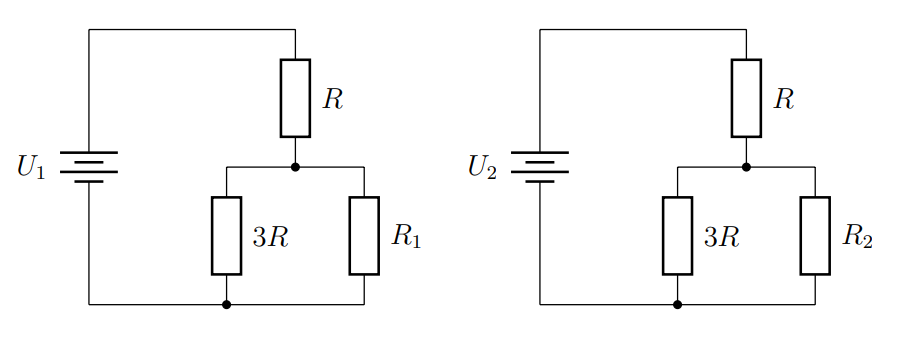
\includegraphics[width=0.5\linewidth]{2015-v3p-06-yl.png}
\end{center}
\fi

\ifHint
Takisti $R_1$ ja takisti $3R$ otstel olev pinge on sama, sest nad on ühendatud paralleelselt. Sama kehtib ka takistite $R_2$ ja $3R$ kohta.
\fi

\ifSolution
Esiteks teame, et kui takisti $R_1$ läbiva voolu tugevus on kaks korda suurem kui voolutugevus läbi takisti $3R$ ja pinge nende otstel on sama, sest nad on ühendatud paralleelselt, siis takistus $R_1$ on kaks korda väiksem kui takistus $3R$. Sama loogika annab, et takistus $R_2$ on viis korda väiksem kui takistus $3R$. Saame võrrandid $\frac{3}{2}R = R_1$ ja $\frac{3}{5}R = R_2$. Nüüd saame leida kahele parallelselt asetatud takistile vastava ekvivalentse takistuse kummalgi skeemil:
\begin{center}
$\frac{1}{R_{ekv1}} = \frac{1}{3R} + \frac{1}{R_1} = \frac{1}{3R} + \frac{2}{3R} = \frac{1}{R}$
\end{center}
\begin{center}
$R_{ekv1} = R$
\end{center}
\begin{center}
$\frac{1}{R_{ekv2}} = \frac{1}{3R} + \frac{1}{R_2} = \frac{1}{3R} + \frac{5}{3R} = \frac{2}{R}$
\end{center}
\begin{center}
${R_{ekv2}} = \frac{R}{2}$.
\end{center}
Saame leida kummalegi skeemile ekvivalentsed takistused: esimese jaoks
\begin{center}
$R + R_{ekv1} = 2R$
\end{center}
ja teise jaoks
\begin{center}
$R + R_{ekv2} = \frac{3R}{2}$.
\end{center}
Viimase asjana teame, et kuna takistit $R$ läbib mõlemal skeemil sama tugevusega vool, siis patareide pinged peavad olema proportsionaalsed just leitud ekvivalentstakistusega. Seega saame, et esimese patarei pinge $U_1$ on suurem kui $U_2$, sest $2R > \frac{3R}{2}$ ning $\frac{U_1}{U_2} = \frac{2R}{\cfrac{3}{2}R} = \frac{4}{3}$.
\fi
}